%   Filename    : chapter_4.tex 
\chapter{Research Methodology}

\section{Research Activities}

\subsection{Information Gathering}
The developers reached out to the College of Arts and Sciences Office of the College Secretary to decide the features and functionality of ReTrac. They asked what type of documents can be requested at their office, the cost for requesting each document, and the process for requesting the documents. The Office of the College Secretary also shared the blog site where the document request form can be downloaded. The document request form is as shown in Figure \ref{fig:requestSlip}.
\begin{figure}[hb!]
  \caption{\label{fig:requestSlip} The request form currently used.}
  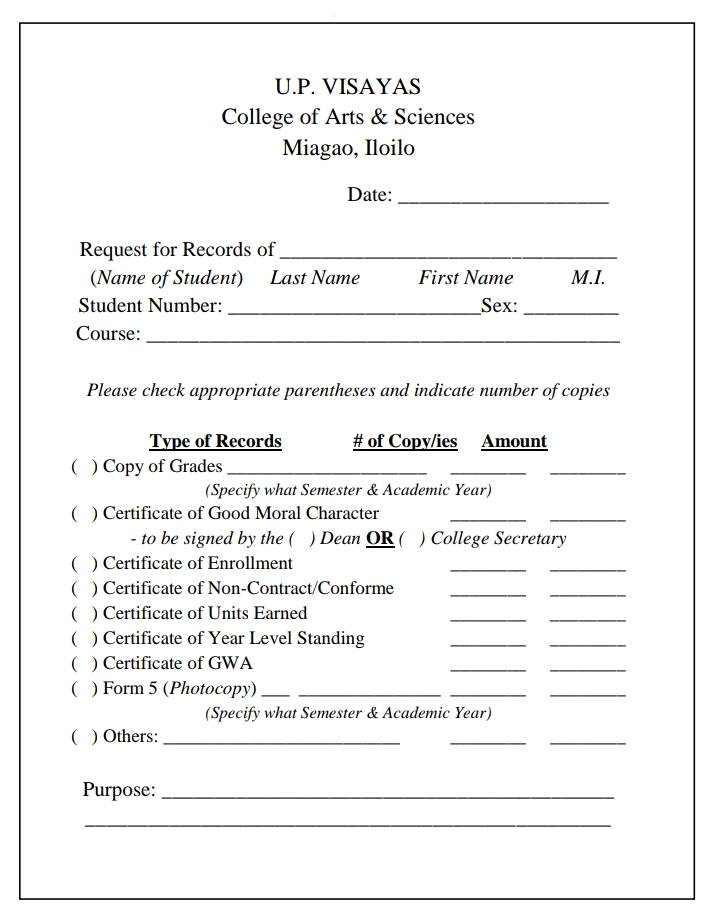
\includegraphics[width=\textwidth]{requestSlip.jpg}
\end{figure}

The developers interviewed Ms. Maureen Kay Ongco, Chief of the University's Cash Office, regarding the payment methods for requesting documents, the payment methods currently being implemented, and the payment methods they are planning to remove and/or add. 

The Cash Office currently supports Land Bank and GCash payment transactions. However, Ms. Ongco elaborated that the GCash payment is only temporary. It was only implemented during the pandemic since some students who request documents do not have bank accounts, specifically that of Land Bank. Ms. Ongco said that the Cash Office is currently negotiating with PayMaya and that PayMaya will be their main payment method when the negotiation pushes through.


\subsection{Application Features}
The application will have the following features:
\begin{itemize}
   \item Students can make document requests
   \item Students can track and see which office handles their request
   \item The students can retrieve the documents they requested
   \item The students can pay through the in-app payment integration
   \item The Office of the College Secretary (OCS) can see the number of pending requests
   \item The OCS can also retrieve and process the request
   \item The OCS can send the documents through the application
   \item The Cash Office can confirm the payment made by the students
\end{itemize}

\subsection{Platform}
There are three options for the application’s platform, (1) desktop, (2) mobile, and (3) web. The pros and cons of each platform are as discussed below.

A desktop application is more accessible for University Offices since they already use desktop computers for their day-to-day tasks. However, not all students have access to desktop computers. Most students own a smartphone that makes mobile applications more accessible to them. On the other hand, web applications can be accessed both on mobile devices and desktop computers through web browsers.

With those considerations, the developers decided to settle with using the web as the platform for the document request and tracking application. Furthermore, developing a version for the desktop and mobile separately would make it more difficult to update feature changes and patches. Developing a web application would also mean that only one application will be maintained making it faster to implement changes.
\subsection{Technology}
The design of the user interface (UI) of the system is done using Figma, a web-based graphics editor and prototyping tool.

The front-end of the system is developed using the React framework. Although there are other Javascript frameworks on the market, the developers are most familiar with React. In addition to the front-end framework, Vitejs is also used. Vitejs is a build tool for React and other frameworks, it also offers tools for enhanced developer experience.

To make the system accessible to users, a cloud service provider is needed. The market offers a wide variety of cloud service, that includes Google Cloud, Amazon AWS, Microsoft Azure, and IBM Cloud among others. There are also services that offers free-tier or trial periods, among which is Firebase. Firebase is a Backend-as-a-Service (BaaS) web technology under Google.

The tools needed for the document request and tracking system includes:
\begin{itemize}
   \item Hosting - a domain to make the website accessible to users
   \item Database - to store documents and information on the web application
   \item Authentication - to secure the application and only allow authenticated users to make and track requests.
\end{itemize}

The tools mentioned above are all present in Firebase. Instead of using multiple cloud services which makes it difficult to manage the web applications dependencies, it is better to use a cloud service that provides all the tools needed for the web application. Moreover, the Spark Plan, which is the free-tier offer of Firebase, can provide enough resources to deploy a big web application.

\subsection{Development Framework}
This study will use the incremental and iterative approach in developing the entire system, specifically, the Scrum Framework in Agile Development. Incremental approach breaks down the system development to smaller tasks and the iterative approach ensures a systematic development cycle through what is called 'iterations'.

Through incremental and iterative approach, the progress is build incrementally and adapting to changes is easier since it is done in iterations.

The Scrum Framework will enable the developers to deliver the minimum viable product (MVP) as early as possible for feedback collection. The said framework would also help given the limited manpower.


\section{Calendar of Activities}

A Gantt chart showing the schedule of the activities should be included as a table. For example:

Table \ref{tab:timetableactivities} shows a Gantt chart of the activities.  Each bullet represents approximately
one week worth of activity.

%
%  the following commands will be used for filling up the bullets in the Gantt chart
%
\newcommand{\weekone}{\textbullet}
\newcommand{\weektwo}{\textbullet \textbullet}
\newcommand{\weekthree}{\textbullet \textbullet \textbullet}
\newcommand{\weekfour}{\textbullet \textbullet \textbullet \textbullet}

%
%  alternative to bullet is a star 
%
\begin{comment}
   \newcommand{\weekone}{$\star$}
   \newcommand{\weektwo}{$\star \star$}
   \newcommand{\weekthree}{$\star \star \star$}
   \newcommand{\weekfour}{$\star \star \star \star$ }
\end{comment}



\begin{table}[ht!]   %t means place on top, replace with b if you want to place at the bottom
\centering
\caption{Timetable of Activities} \vspace{0.25cm}
\begin{tabular}{|p{2in}|c|c|c|c|c|c|c|c|} \hline
\centering Activities (2009) & Jan   & Feb & Mar & Apr & May & Jun & Jul \\ \hline
Study on Prerequisite Knowledge      &   &  & ~~~\weektwo & \weekfour &  &  &  \\ \hline
Review of Existing Racing Strategies & ~~~\weektwo  & \weekfour & \weekfour & \weekfour &  &  &  \\ \hline
Identification of Best Features      &   &  &  & \weekfour & \weektwo~~~ &  &  \\ \hline
Development of Racing Strategies     &   &  &  & ~~~\weektwo & \weekfour & \weektwo~~~ &  \\ \hline
Simulation of Racing Strategies      &   &  &  & ~~~\weektwo & \weekfour & \weekthree~~ &  \\ \hline
Analysis and Interpretation of the Results &   &  &  &  & \weekfour & \weekfour & \weekone~~~~~ \\ \hline
Documentation & ~~~\weektwo  & \weekfour & \weekfour & \weekfour & \weekfour & \weekfour & \weektwo~~~ \\ \hline
\end{tabular}
\label{tab:timetableactivities}
\vspace{0.1cm}
\flushright{$\bullet$ indicates the number of weeks}
\end{table}


